% !TeX encoding = UTF-8
% !TeX spellcheck = es_ES
% !TeX root = ../ComponentCatalog.tex
%!TEX root=../ComponentCatalog.tex
%Modulo Rele
\begin{table}[H]
    \centering
    \renewcommand\theadfont{\bfseries}
    \setlength{\tabcolsep}{10pt}
    \renewcommand{\arraystretch}{1.5}

    \begin{tabular}{|c|c|c|c|c|}
        \beginConnectorTable{Keypad Capacitivo}
        \multirow{6}{*}{\makecell{16 Keys \\ TTP229}}
        \connectordata[6]{
            %\draw (0,0) rectangle  +(2.5,1.8);
            \begin{scope}
                \clip (0,0) rectangle  +(3,3);
                \node[inner sep=0pt] at (1.4,1.5)
                    {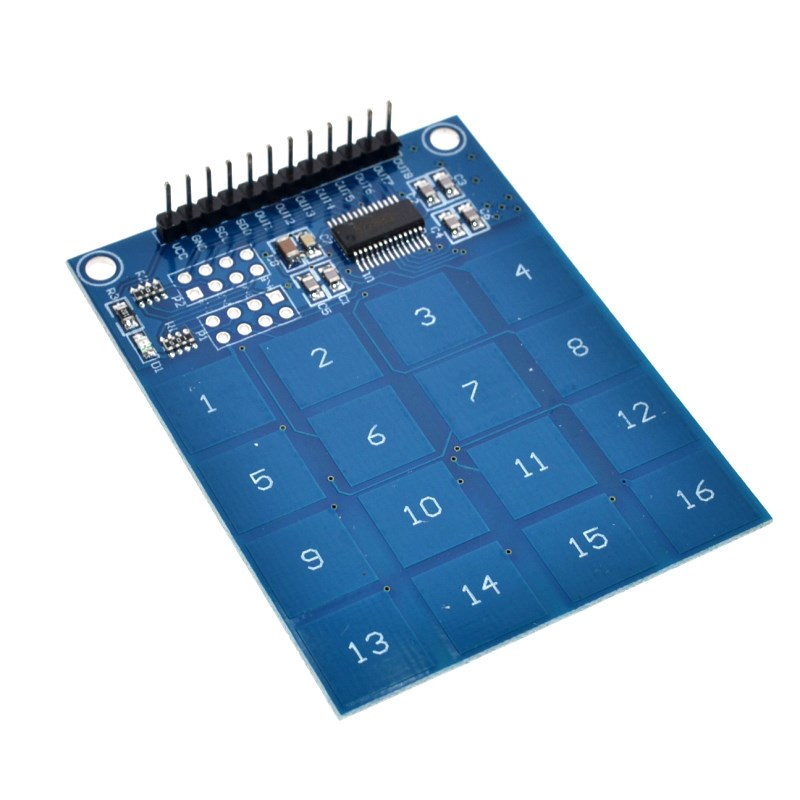
\includegraphics[scale=.15]{pictures/KP_Capa.jpg}};
            \end{scope}
        }{
            \draw (0,0) rectangle (3,1.5) ;
        }{Aliexpress}{ttp229 Keypad} {5V} {10mA}
        \cline{1 - 2}
        \connectorblockinfo{Uso}{KeyPad mando LCB}
        \connectorblockinfo{Ubicacion}{TT-Tren}
    \end{tabular}
    \caption{KeyPads}
    \label{tab:ttp229-keypad}
\end{table}